\chapter{Cross Domain Learning For Online Advertisement}
\label{chapterlabel5}
\section{Transfer Learning and Domain Adaptation}
Traditional supervised learning is relied on the assumption that the distribution of training and test instances are similar. However, it is rare in real life that the distributions among datasets are unchanged. As discussed in \cite{facebook2015}, many proposed machine learning algorithms and models can be only used under the assumption that the training and test datasets are derived from the same distribution and with same feature space, when the distribution changes, new data needs to be collected and new model needs to be rebuilt. For the industry of online advertisement, it is expensive and time-consuming to rebuild the model, in this case, transfer learning is needed which can borrow the knowledge learned from previous advertisement campaigns and apply to new campaigns to increase the efficiency for CTR prediction and decrease the cost for training new model. According to the research in \cite{pan2008transfer}, the behaviors of users among different campaigns are volatile and unpredictable, in traditional statistical machine learning problem, it is based on the ideal assumption that the model learned will not affect the real world, independent and identically distributed samples on different campaigns ensures the generalization. However when it comes to the real-world online advertisement industry, after the model is introduced into production, the users behavior will be affected, and also the distribution of the data. In brief, the changeable user behaviors among online advertisement campaigns determine that static statistical model is not suitable for dynamic online advertisement CTR prediction, \textit{transfer learning} is desirable which can save significant time and effort. 

\begin{figure}[t]
\centering
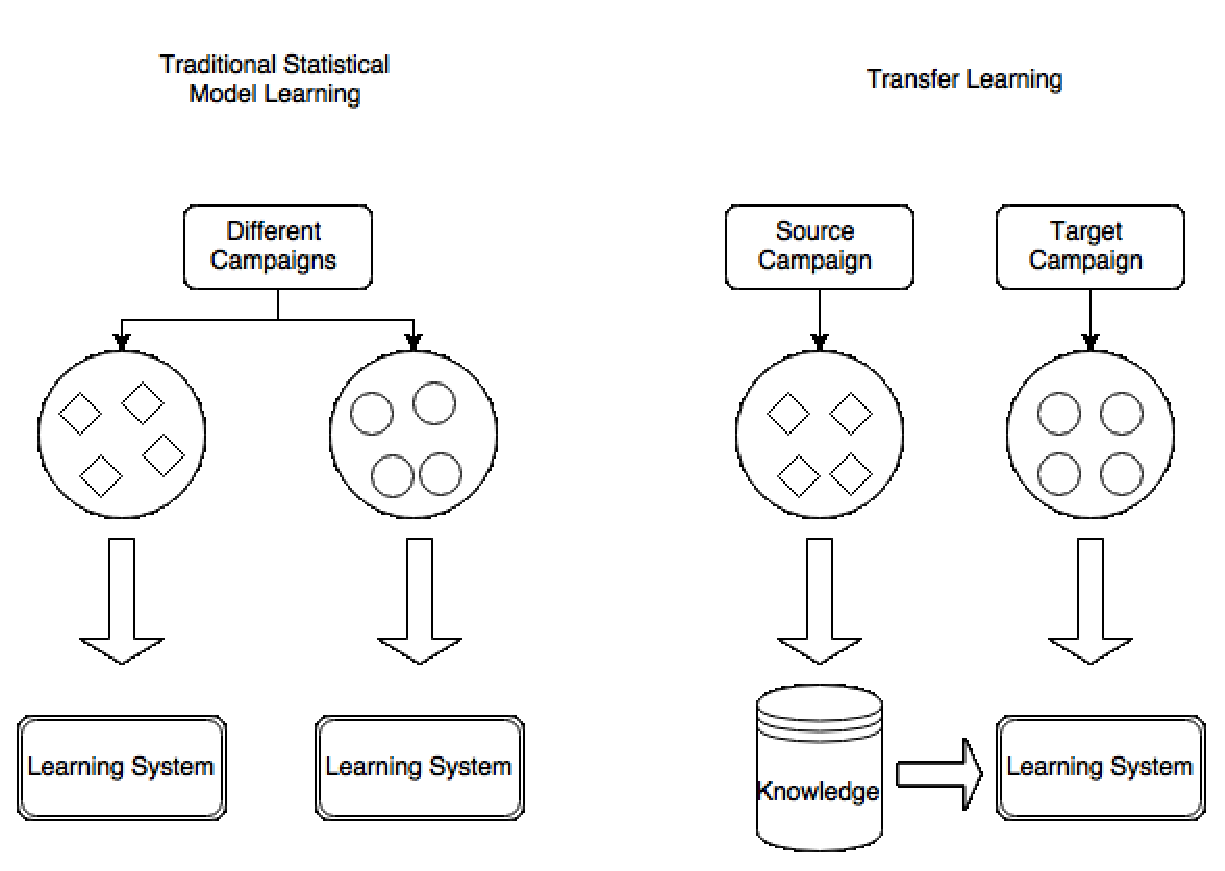
\includegraphics[width=\columnwidth]{transferlearning.eps}
\caption{Different Learning system between traditional machine learning and transfer learning}
\label{fig:transfer}
\end{figure}

At first, using the definitions in \cite{pan2010survey}, we specify \textit{domain} \textit{D} as each campaign's impressions raw data, and \textit{task} \textit{T} as the learning system of the model, in which, \(D = \{X,P(X)\}\), also  \(D = \{Y,P(Y|X)\}\). \(X = \{x_1,x_2, ..., x_n\}\) in which \(x_i\) is one impression in the campaign, and \(Y = \{y_1,y_2, ..., y_n\}\) is the label for each impression, namely whether in this impression the click occurs. The training data is composed of the pairs of \(\{x_i,y_i\}\) which can be used to train the model, and the conditional distribution \(P(Y|X)\). We define \textit{source domain} as the old campaign and \textit{target domain} as the new campaign, then \(X_s\) will be the feature space of source domain and \(P(X_s)\) is the marginal probability distribution of the feature space of source domain, similar, \(X_t\) will be the feature space of target domain and \(P(X_t)\) is the marginal probability distribution of the feature space of target domain. \(Y_s\) is the class label of the features in source domain and \(Y_t\) will be the corresponding label for target domain. By considering the relation between source domain and target domain, as well as source task and target task, the model learning problem can be classified as follows in the scope of online advertisement. 

\begin{enumerate}
\item if \(D_s = D_t\) and \(T_s = T_t\), this is a traditional machine learning problem. For example, the source and target advertisement campaigns follow the same distribution, and their learning tasks are the same, which are to predict the CTR based on the feature spaces. 

\item if  \(D_s \neq D_t\) and \(T_s = T_t\), which means the source and target domains are distinct but with the same tasks. The problem is also known as \textit{domain adaptation} \cite{arnold2007comparative} since the two domains are different in the marginal probability distribution but same for tasks. This situation can be further classified into two types:
    \begin{itemize}
    \item  \(X_s \neq X_t\), which means the feature spaces of the two domains are different with each other, for example, one domain of an advertisement campaign  \textit{International e-commerce} and the other is from \textit{ Software} as shown in \cite{zhang2014real}, if the impressions of the two domains are encoded into binary feature, surely there will be small overlap between the two feature spaces and the feature spaces will be largely different.
    \item \(P(X_s) \neq P(x_t) \), which means the probability distributions of the two advertisement campaigns are different, so they are from different fields, with different themes. 
    
    \end{itemize}
\item if  \(D_s = D_t\) and \(T_s \neq T_t\), it can also be classified into two types:
     \begin{itemize}
    \item  \(Y_s \neq Y_t\), this means the label spaces are different for two domains, as an example for online advertisement, the label in one domain could be click/non-click, which is dichotomic, but in the other domain the labels can be winning price, which is continuous.
    \item \(P(Y_s|X_s) \neq P(Y_t|X_t) \), this means the conditional probability distributions of the label on feature spaces are different for two domains, one example can be due to the existence of online robots, for one campaign all the impressions are randomly clicked or seen by programs, but the other campaign successfully prevent themselves from the robots so all clicks are effective and valid which simulates the human behaviors in the real world.  
  \end{itemize}
\end{enumerate}

In this paper, we will focus on transductive transfer learning, or \textit{domain adaptation}, since our learning task is obvious, which is CTR prediction, and we assumes that the robots are rare in the campaign, so the conditional probability are similar between the two campaigns, since the similar human behaviors will lead to similar advertisement clicking actions. 

As discussed above, domain is composed of feature space and feature probability distribution. In this paper, since our goal is to compare the performance of binary feature and counting feature, so we will represent the feature space and feature probability distribution of source and target domain in Table~\ref{tab:domainadapt}.

\begin{table}[h]
\centering
\begin{tabular}{ c | l | l }
Feature Types & Feature Space & Feature Distribution \\
\hline \hline
Binary Feature & Different & Different  \\
Counting Feature & Same & Different
\end{tabular}
\caption{Source and Target domain comparison for Binary and Counting Features}
\label{tab:domainadapt}
\end{table}

To clarify, for binary feature, suppose in the user dataset of online advertisement there is a categorical feature \textit{nationality}, with the value \textit{China}, \textit{UK}, \textit{USA}, etc. It is not surprising that the original field space will be blew up to hundreds of features which is the number of countries in the world, without pre-processing, we even cannot distinguish \textit{UK} from \textit{Great Britain}, which makes astronomical number of features with the increasing of new impressions. Microsoft claims that they have hundreds of millions features \cite{graepel2010web} for each training dataset, as we are already in the age of big data online advertisement, we can expect that the data volume will increase to the magnitude of hundred billion with hundred billion sparse discrete features. Even for our experiment, millions of features will arise from the dataset when the number of impressions reach 1 million. Therefore, the feature spaces are always distinct between the old campaigns and new campaigns. 

Therefore, in this part we will discuss on how to apply a classifier trained on the old advertising campaigns, or source domains for the use in the new campaigns, or target domain. Since the distribution between the features in the source domain and target domain are different, we expect that the more similar the two distributions are, the better performance the classifier trained on the source domain will have on the target domain. As we said above, we define a distribution of a domain as \(D\) on the instance set \(X\), which are different from domain to domain, however, the tasks are the same in multiple domains. So what we propose here is as follows:
\begin{itemize}
  \item \(D_s \neq D_t\), and \(X_s \neq X_t\). This is not surprising since for advertisement campaigns, normally there is not a huge overlap among the two domains.  
  \item \(T_s = T_t\) which means that the learning tasks are the same for the two domains.
\end{itemize}
Therefore, we will be faced up to the following three problems:
\begin{enumerate}
  \item How to measure the variance between two domains ? Namely how to find the relation between \(D_s\) and \(D_t\) and to say they can be regarded as the same ?
  \item Whether we can directly apply the classifiers learned from source domain to target domain ? Instead of using probit distribution to represent weights space and update the weights with the new come-in data as an active learning problem, as discussed in \cite{graepel2010web}, we hope to find a baseline that even though without updating the weights but directly using the old weights space, whether we can still obtain decent CTR prediction performance ? Namely whether we can regard \(Pr(y_s|x_s)\) as the same of \(Pr(y_t|x_t)\) considering that \(X_s \neq X_t\) ? 
\end{enumerate}



\section{Advertisement Campaign Datasets Shift}
In this part, we will discuss on the relation between the distributions among different domains. Normally, the relation between two domains can be represented using the indicators in 
\cite{shen2015effective}:
\begin{itemize}
\item Similarity : A score which looks at how similar
the two domains are. In terms of probability model.
\item Novelty : A score which the additional part generated from the target domain which does not exist in the source domain.
\end{itemize}
The relation can be shown in Figure ~\ref{fig:crossdomain}
\begin{figure}[h]
\centering
\includegraphics[width=\columnwidth]{crossdomain.png}
\caption{Similarity and Novelty in Source and Target Domains}
\label{fig:crossdomain}
\end{figure}
Intuitively, we know that the bigger the novelty is, the harder that we can apply our classifiers into the new campaign. So we should find a method to measure the similarity and novelty between two domains. 
\cite{bickel2009discriminative} proposes the concept of \textit{Covariate Shift}, which shows the case that distribution generating the new data to be tested varies from the distribution that generating the data used to train the model, therefore the new inputs used as predictors will change between training and testing stages. To simplify, \(P(X_s) \neq P(X_t)\).

In order to measure the covariate shift between domains, I devised a simple method to quickly detect the similarity and novelty, the basic idea is that, given two domains, if their feature distributions are nearly identical to each other, we would be hard to distinguish between them if we mix them together. On the other hand, when the distribution differ to each other, it will be capable to predict the label of the two domains. So a basic experiment is designed as follows:
\begin{itemize}
\item For the source domain, we remove its label of \textit{click}, but add a new label \textit{source} to each impression to show that the source domain is \textit{source} dataset.
\item For the target domain, we also remove its label for clicks but add a new label \textit{target} to show they belong to another dataset
\item Mix the two dataset together and use 10 fold cross validation method to train a model using a sample of the data and use the rest of the data as test to predict the label of dataset.
\item After 10 times of trial, for each pair of source and target domains, we can get the mean RMSE and regard it as the final RMSE between the two domains, the higher the RMSE, the harder that the classifiers to predict the label of the two datasets, showing that the two domains are hard to distinguish, and the distributions of them are more similar.
\item We use the idea proposed in \cite{ben2010theory}, as the \textit{transfer distance}, or \textif{Proxy-A-distance} (PAD) to measure how two domains are different to each other, the metric is defined as:
\begin{equation}
A distance = 2 \times (1-2 \times \epsilon)
\end{equation}
in which \(\epsilon\) is the generalization error of a classifier to distinguish the labels of the input data, here we use RMSE to represent it. So the lower the \textit{A-distance} is, the similar the two domains are.

Since we have 10 campaigns from the Adform dataset, for each dataset, we calculate its \textit{A-distance} with all other 9 campaigns to get a vector of 9 A-distance, and obtain the mean and variance value of this vector, the result is in Figure \ref{fig:beforeall}.

\end{itemize}
\begin{figure}[h]
\centering
\includegraphics[width=\columnwidth]{beforesigmoidall.png}
\caption{Mean and Variance value of A-distance sets of one campaign to the other 9 campaigns}
\label{fig:beforeall}
\end{figure}

From Figure ~\ref{fig:beforeall} we can see that the \textit{A-distance} are big and varies in a big range. Especially for counting feature the feature spaces of the 10 campaigns differ from each other dramatically. It is not surprising since counting feature is able to transfer the variability in the weights space to feature space, so the weights space of counting feature are much more similar to each other than binary feature. We can conclude from this part that \(Pr(x_s) \neq Pr(x_t)\)

\section{Cross Dataset Generalization}
The lucky thing is that based on the Bayesian format of logistic regression model,

\begin{equation}
Pr(y|x,w) = \frac{Pr(w|x,y)*Pr(y|x)}{Pr(w)}
\end{equation}

in which 
\begin{equation}
sigmoid = \frac{1}{1 + \exp(-w^T x)} 
\end{equation}

we can know that the inference of logistic regression is not based on \(Pr(x)\), but on \(Pr(y|x)\) largely. 

Then we can transform the feature space \(x\) into a new logistic space \(sigmoid(x^T*w)\) when \(y = 1\) which is as follows:



\begin{bmatrix} 
sigmoid(w_1*x_{11}) & sigmoid(w_1*x_{12}) .... & sigmoid(w_n * x_{1n})\\
sigmoid(w_1*x_{21}) & sigmoid(w_1*x_{22}) .... & sigmoid(w_n * x_{2n})\\
......\\
sigmoid(w_1*x_{N1}) & sigmoid(w_1*x_{N2}) .... & sigmoid(w_n * x_{Nn})
\end{bmatrix}

And using the same method as above, the similarities among the logistic spaces can be shown as follows:
\begin{figure}[h]
\centering
\includegraphics[width=\columnwidth]{aftersigmoid.png}
\caption{Mean and Variance value of A-distance sets of one campaign to the other 9 campaigns for y-space}
\label{fig:after1}
\end{figure}

It can be seen that in most cases the A-distance between the source domain to the rest of the targets domains are quite low, so \(Pr(y_s|x_s) = Pr(y_t|x_t)\) is a reasonable assumption.

Therefore, we can directly apply the model learned from old campaign to the new campaign and we are expected to still get decent CTR prediction performance, what's more, since the counting value of counting feature model can take over the variability between old and new campaigns, by updating the counting value, we can gradually transform the distribution of old campaign \(Pr(x_s)\) to \(Pr(x_t)\) with increasing number of new incoming data, thus outperforming binary feature considerably after several updates. 